% !TEX program = xelatex
% =====================================================================
%  七张教学插图解析
%  逐张说明图画了什么、数据从哪来、怎么看、能证明什么
%  编译：xelatex 图解析.tex （连续两遍）
% =====================================================================
\documentclass[11pt,a4paper]{article}
\usepackage[UTF8]{ctex}
\usepackage{amsmath,amssymb}
\usepackage{geometry}
\usepackage{graphicx}
\usepackage{booktabs}
\usepackage{longtable}
\usepackage{array}
\usepackage{enumitem}
\usepackage{xcolor}
\usepackage{listings}
\usepackage{caption}
\usepackage{float}
\usepackage[hidelinks]{hyperref}

\geometry{left=2.2cm,right=2.2cm,top=2.5cm,bottom=2.5cm}
\linespread{1.30}
\setlength{\parskip}{4pt}
\setlength{\tabcolsep}{5pt}
\captionsetup{font=small,labelfont=bf}
\graphicspath{{../详解/fig/}}
\setmonofont{Consolas}

\lstset{
  language=Python,
  basicstyle=\ttfamily\small,
  breaklines=true,
  columns=flexible,
  keepspaces=true,
  frame=single,
  framexleftmargin=2pt,
  xleftmargin=8pt,
  showstringspaces=false,
  commentstyle=\color{black!55},
  keywordstyle=\bfseries,
  extendedchars=true,
  numbers=left,
  numberstyle=\tiny\color{gray},
}

\newcommand{\keypoint}[1]{%
  \begin{center}
  \fcolorbox{black!55}{black!4}{%
    \begin{minipage}{0.94\textwidth}
    \vspace{2pt}\textbf{一句话结论}\quad #1\vspace{2pt}
    \end{minipage}}
  \end{center}}

\title{\bfseries 七张教学插图解析\\[6pt]
\large 每张图画了什么、数据从哪来、怎么看、能证明什么}
\author{}
\date{\today}

\begin{document}
\maketitle
\thispagestyle{empty}

\vspace{0.6em}
\noindent
\textbf{这份文档做什么。}
它把讲解稿里的七张插图逐张拆开讲清楚：
这张图想回答什么疑问、画的是什么、数据从哪来、
图上每一个元素怎么读、能读出哪些数、
这张图能证明什么、不能证明什么、生成它的代码长什么样。

\vspace{4pt}
\noindent
\textbf{为什么要单独讲图。}
图比文字更容易被误读。同一张图，
作者想让你看的是趋势，读者可能盯着某条线的绝对高度；
作者用的是实算数据，读者可能以为是示意图。
把每张图的来源和读法写清楚，图才真的有用。

\vspace{4pt}
\noindent
\textbf{七张图的清单。}
编号、文件名、类型与出处如下表。类型分三种：
示意图是按公式或几何关系画出来的，不含求解器输出；
数据图是把求解器的计算结果画出来；
引用数据图指图中的数据不是本次实算，而是取自既有报告。

\begin{center}
\small
\begin{tabular}{@{}cllll@{}}
\toprule
编号 & 文件 & 图名 & 类型 & 出现在讲解稿 \\
\midrule
图 1 & fig\_cv.png & 控制体与两种径向离散 & 示意图 & 第一部分 \\
图 2 & fig\_p1.png & 问题一温度与水分剖面 & 数据图 & 第一部分 \\
图 3 & fig\_map.png & 坐标变换的几何意义 & 示意图 & 第二部分 \\
图 4 & fig\_cheb.png & 切比雪夫节点的来源 & 示意图 & 第二部分 \\
图 5 & fig\_p3.png & 问题三干燥曲线与终点放大 & 数据图 & 第二部分 \\
图 6 & fig\_flux.png & 通量形式的谱配置 & 示意图 & 第三部分 \\
图 7 & fig\_conv.png & 两种离散方式的收敛对比 & 数据图加引用数据 & 第四部分 \\
\bottomrule
\end{tabular}
\end{center}

\vspace{4pt}
\noindent
\textbf{复现方式。}
全部七张图由同一个脚本 \texttt{figs.py} 生成，
在讲解稿目录下执行 \texttt{python figs.py} 即可重新得到，
输出写入 \texttt{fig} 子目录。
脚本依赖 numpy 与 matplotlib，不需要其他第三方库。

\newpage
\tableofcontents
\newpage

% =====================================================================
\section{画图脚本的三个约定}

在逐张讲图之前，先交代三个贯穿全部插图的约定。

\subsection{中文字体}

matplotlib 默认字体不含汉字，直接画中文会显示成方框。
脚本在开头显式加载 Windows 自带的微软雅黑：

\begin{lstlisting}
FP = r"C:\Windows\Fonts\msyh.ttc"
if os.path.isfile(FP):
    fm.fontManager.addfont(FP)
    plt.rcParams["font.sans-serif"] = ["Microsoft YaHei"]
plt.rcParams["axes.unicode_minus"] = False
\end{lstlisting}

第 1 行给出字体文件的绝对路径，前面的 \texttt{r} 表示原始字符串，
路径里的反斜杠不当作转义字符。
第 2 行到第 4 行先检查文件是否存在，存在就把这个字体注册进 matplotlib，
并把它设成首选无衬线字体。
第 5 行关掉 Unicode 负号，否则负号会因为字体缺字形而显示成方框。

这里有一个可移植性问题值得一提。
代码包的其余脚本都做到了目录搬迁后仍能运行，
而这一段写死了 Windows 字体路径。
换到 Linux 或 macOS 上运行时需要改这一行。
之所以这样写，是因为画图是本地交付环节，不是计算环节，
写死路径比让字体缺失导致图里全是方框更稳妥。

\subsection{绘图后端}

脚本第一行设置后端为 Agg：

\begin{lstlisting}
import matplotlib
matplotlib.use("Agg")
import matplotlib.pyplot as plt
\end{lstlisting}

Agg 是不弹窗口的绘图后端，只把图写成文件。
这样做有两个好处：在没有图形界面的环境里也能跑；
批量生成七张图时不会因为弹窗而中断。

\subsection{分辨率与尺寸}

\begin{lstlisting}
plt.rcParams["savefig.dpi"] = 220
plt.rcParams["figure.dpi"] = 220
\end{lstlisting}

分辨率设成每英寸 220 点。讲解稿是 A4 纸，
插图宽度约十六厘米，换算过来横向有一千三百多个像素，
打印和屏幕阅读都够清楚。

图幅尺寸在每张图里单独指定，多数是宽九点六英寸、高三点五英寸的双栏图，
即左右两个子图。少数是单图，例如图 6 的通量形式示意图。

% =====================================================================
\section{图 1：控制体与两种径向离散}

\begin{figure}[H]
\centering
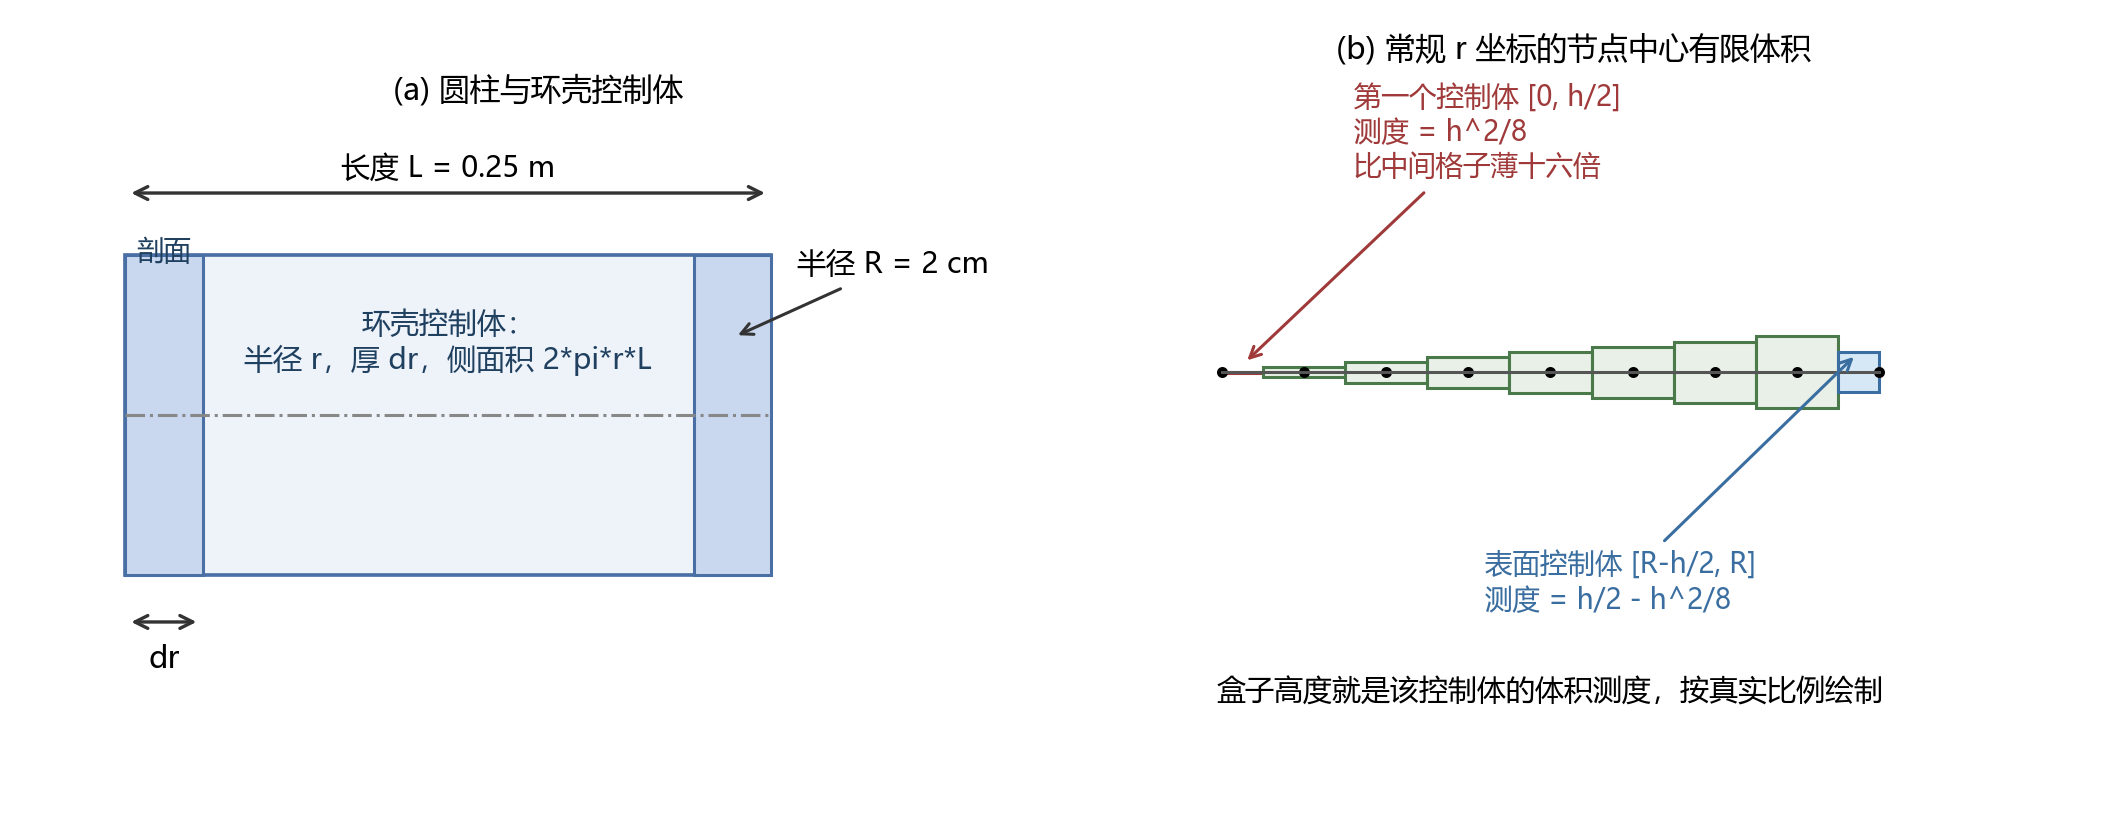
\includegraphics[width=\textwidth]{fig_cv.png}
\caption{控制体与两种径向离散。左图是圆柱与环壳控制体的几何；
右图是常规半径坐标下的节点中心有限体积网格，盒子高度等于该控制体的体积测度。}
\end{figure}

\subsection{这张图回答什么疑问}

读控制方程推导时最容易卡住的地方是两个：
为什么方程里会多出一个半径 $r$，以及为什么不用半径坐标直接离散。
这张图就是为了回答这两问。

\subsection{画的是什么}

左图是圆柱的剖面。中间那条点划线是轴，
从轴到外表面画了一个箭头，标注半径两厘米；
上方箭头标注长度二十五厘米。
图中间的文字说明控制体的取法：
取半径从 $r$ 到 $r+\mathrm{d}r$ 的一层薄壳，厚度标在左下角。

右图把常规半径坐标下的网格画了出来。
归一化半径 $\xi$ 从零到一被等分成八格，每个格子的中点放一个节点。
每个控制体用一个矩形表示，\textbf{矩形的高度等于该控制体的体积测度}，
所以高度是真实比例，不是随手画的。

\subsection{数据从哪来}

这是示意图，不含任何求解器输出。
所有几何量都按定义直接算出：步长 $h$ 等于八分之一，
第一个控制体覆盖零到 $h/2$，测度是 $h^2/8$；
中间第 $i$ 个控制体覆盖 $\xi_i-h/2$ 到 $\xi_i+h/2$，测度是 $\xi_i h$；
最后一个控制体覆盖 $1-h/2$ 到一，测度是 $h/2-h^2/8$。

这三个测度加起来等于二分之一，可以当场验算：
$h^2/8$ 加上 $\sum_{i=1}^{7}\xi_i h$ 再加上 $h/2-h^2/8$。
取 $h=1/8$，第一项是 $1/512$，中间七项之和是 $28/64$，第三项是 $1/16-1/512$，
三项相加正好是 $1/2$。
这个二分之一不是巧合，它来自
$\int_0^1 \xi\,\mathrm{d}\xi=1/2$，也就是环面积与半径成正比的积分结果。

\subsection{逐要素读图}

\begin{itemize}[leftmargin=1.6em]
\item 左图里两个浅色竖条表示薄壳的剖面，中间大块是药材内部。
\item 左图下方的双向箭头标注 $\mathrm{d}r$，表示薄壳厚度趋于零。
\item 右图的横轴是归一化半径，从轴心零到表面一。
\item 右图纵向的盒子高度依次为：第一条极薄，中间逐渐变高，最后一条略低。
\item 红色的短箭头指向最薄的那一条，标注它的测度是 $h^2/8$，
      并说明它比中间格子薄十六倍。
\item 蓝色箭头指向最右边那一条，标注它的测度是 $h/2-h^2/8$。
\item 每个盒子中间的小圆点是节点，节点之间的竖线是控制体界面。
\end{itemize}

\subsection{能读出什么}

\begin{center}
\begin{tabular}{@{}lll@{}}
\toprule
量 & 表达式 & 取 $N=8$ 时的值 \\
\midrule
第一个控制体的测度 & $h^2/8$ & $0.00195$ \\
中间第 $i$ 个控制体的测度 & $\xi_i h$ & 从 $0.0156$ 增到 $0.1094$ \\
最后一个控制体的测度 & $h/2-h^2/8$ & $0.06055$ \\
三个部分之和 & 恒等于 $1/2$ & $0.5$ \\
\bottomrule
\end{tabular}
\end{center}

\subsection{能证明什么，不能证明什么}

这张图能说明的是：半径坐标下的离散必须为轴心单独设计控制体，
第一个控制体只覆盖半格，测度是 $h^2/8$，
比中间格子小一个多数量级；表面那个控制体也要单独处理。
这两处特殊处理正是半径坐标离散复杂度的来源。

它不能说明谱方法有多准，也不能说明新坐标变换的效果。
那些要用图 7 来回答。

\subsection{生成代码}

右图的画法如下。盒子高度直接取上面三个测度表达式，
所以图上的几何比例与公式完全一致。

\begin{lstlisting}
N = 8
h = 1.0 / N
for i in range(N + 1):
    x = i * h
    if i == 0:
        w = h * h / 8.0
        b.add_patch(Rectangle((0.0, -w / 2), h / 2, w, ...))
    elif i == N:
        w = h / 2 - h * h / 8
        b.add_patch(Rectangle((1 - h / 2, -w / 2), h / 2, w, ...))
    else:
        w = x * h
        b.add_patch(Rectangle((x - h / 2, -w / 2), h, w, ...))
    b.plot([x], [0], "ko", ms=2.6)
\end{lstlisting}

第 1 行与第 2 行把归一化半径分成八格，步长是八分之一。
第 3 行到第 12 行按三种情形分别画盒子。
第 4 行到第 6 行处理第一个控制体：宽度是半格，高度是 $h^2/8$。
第 7 行到第 9 行处理最后一个控制体。
第 10 行到第 12 行处理中间的控制体，高度是 $\xi_i h$。
第 13 行在每格中点画节点。

\subsection{容易读错的地方}

第一个控制体在图上是极薄的一条，容易被当成画错了。
它不是画错，而是这个控制体本来就极小：
在 $N=8$ 时它比中间格子薄十六倍，节点加密以后差距还要按平方拉大。
这张图的意义正在于显示这一点。

另外要注意，右图画的是常规半径坐标的离散，不是本文采用的方法。
本文在 $u=(r/R)^2$ 坐标下离散，那个坐标下不需要任何特殊控制体，
这也正是选择新坐标的原因。

% =====================================================================
\section{图 2：问题一温度与水分剖面}

\begin{figure}[H]
\centering
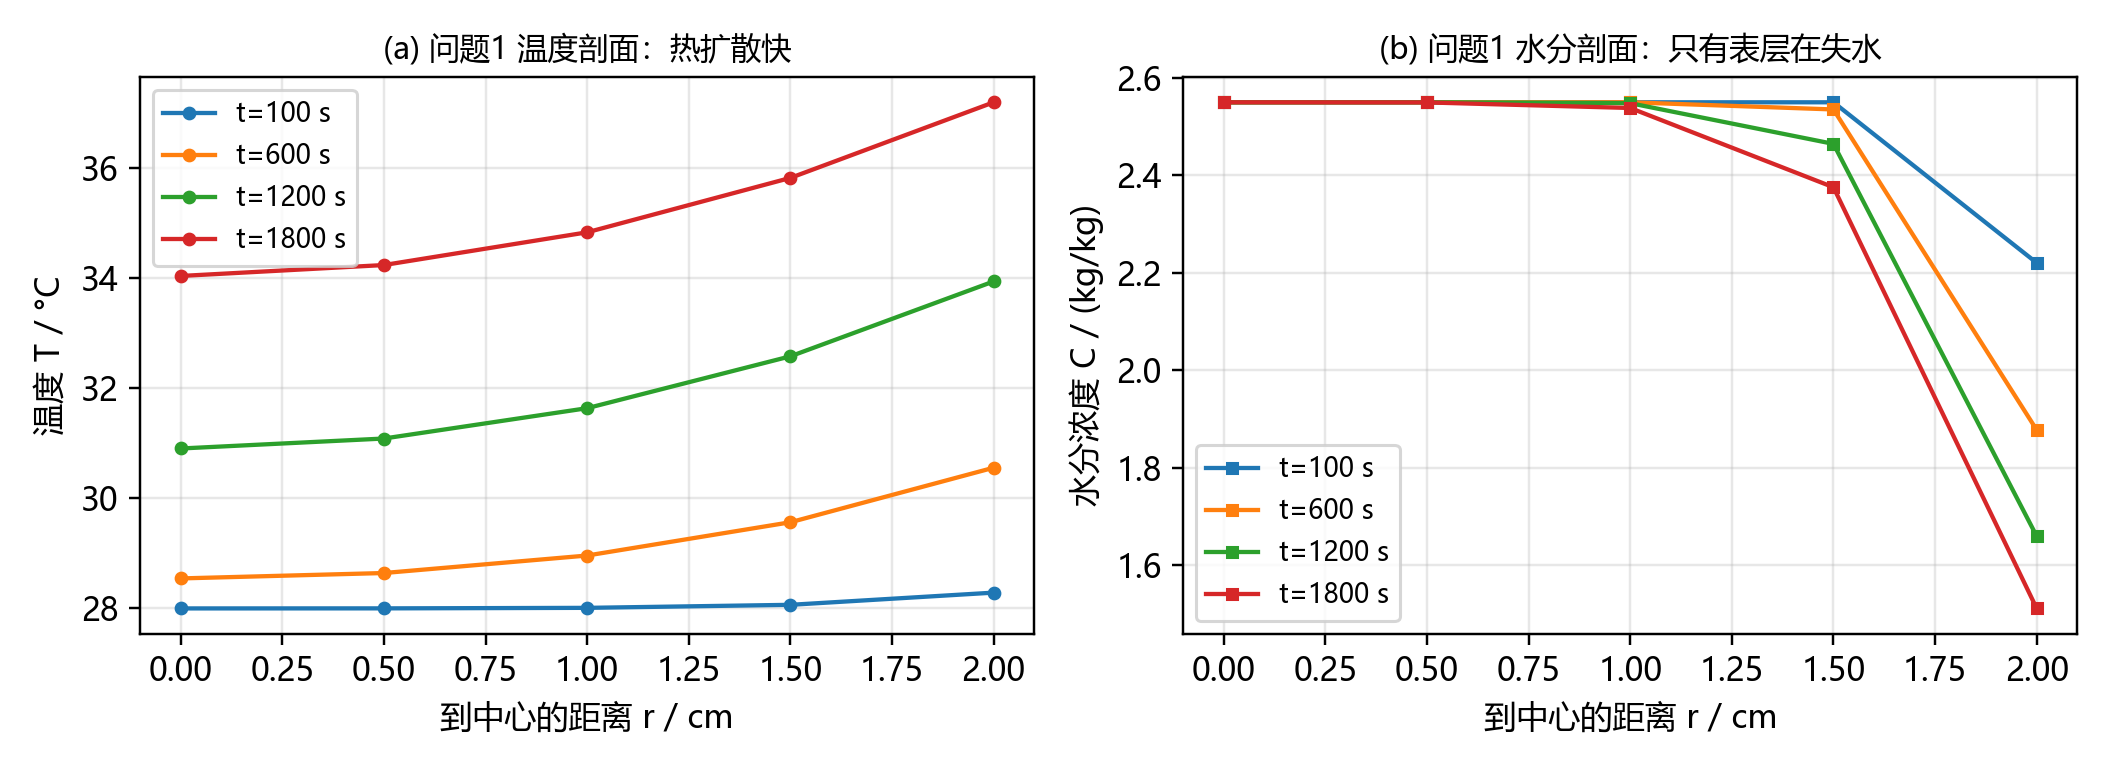
\includegraphics[width=\textwidth]{fig_p1.png}
\caption{问题一的温度剖面与水分剖面演化。
左图四条曲线对应四个时刻的温度分布，右图同样四个时刻的水分分布。}
\end{figure}

\subsection{这张图回答什么疑问}

温度与水分都在扩散，为什么两者的演化速度差这么多。
这张图用同一条时间轴把两个场并排画出来，
让差别直接可见。

\subsection{画的是什么}

两个子图共用横轴：到药材中心的距离，从零到两厘米。
左图的纵轴是温度，单位摄氏度；右图的纵轴是水分浓度，单位千克每千克。
每个子图画四条曲线，对应一百秒、六百秒、一千二百秒、一千八百秒四个时刻。

\subsection{数据从哪来}

数据由主求解器实算，参数是节点数六十四、问题一物性、
相对容差 $10^{-11}$、含水率绝对容差 $10^{-13}$、温度绝对容差 $10^{-11}$。
时间网格从零到一千八百秒，间隔六十秒，共三十一个时刻。
每个时刻把节点上的解用重心插值到五个目标半径零、零点五、一、一点五、两厘米，
再把这五个点连成曲线。

这里有一个细节值得说明：图上每条曲线只有五个数据点，
看起来却像光滑曲线，是因为 matplotlib 把相邻点用直线连起来了。
不要以为曲线中间的细节有物理含义，
真正的解是在五十六个以上的节点上算出来再插值到这五个位置的。

\subsection{逐要素读图}

\begin{itemize}[leftmargin=1.6em]
\item 左图四条曲线自上而下依次对应时刻由晚到早，温度随时间整体抬升。
\item 左图里同一时刻表面温度高于中心温度，说明热量从表面传入。
\item 右图四条曲线在靠近轴心处几乎重合，都贴着初值 $2.55$。
\item 右图里只有最右侧一段随时刻明显下降，说明失水集中在表层。
\item 右图最下方那条曲线在 $r=2$ 厘米处降到一点五左右，
      而同一时刻中心还停在初值附近。
\end{itemize}

\subsection{能读出什么}

四个时刻的关键读数如下，单位分别是摄氏度和千克每千克。

\begin{center}
\begin{tabular}{@{}lrrrr@{}}
\toprule
时刻 / 秒 & 中心温度 & 表面温度 & 中心含水率 & 表面含水率 \\
\midrule
100 & 28.0003 & 28.2875 & 2.550000 & 2.2204 \\
600 & 28.5456 & 30.5576 & 2.550000 & 1.8773 \\
1200 & 30.9069 & 33.9433 & 2.550000 & 1.6591 \\
1800 & 34.0425 & 37.1989 & 2.5500 & 1.5109 \\
\bottomrule
\end{tabular}
\end{center}

从这张表还能读出两个有意义的量。
第一是同一时刻中心与表面的温差：
一百秒时只有零点二九摄氏度，六百秒时二点零一，一千二百秒时三点零四，
一千八百秒时三点一六摄氏度。温差先快速拉开，之后增速变慢。
第二是表面水分从初值降下来的幅度：
四个时刻分别是零点三三、零点六七、零点八九、一点零四，
而中心在一千八百秒时只降了不到万分之一。

为什么差这么多，可以用特征时间判断。
温度的特征时间是 $R^2/\alpha$，等于两千三百六十九秒；
水分的特征时间是 $R^2/D$，取初值处的扩散系数，等于八万一千秒。
后者是前者的三十四倍。
所以三十分钟这段时间里，温度场已经明显变化，水分场还没来得及动。

\subsection{能证明什么，不能证明什么}

这张图能说明热快质慢这个物理图像，
并且为后面两个问题埋下伏笔：
干燥的瓶颈在内部扩散，不在表面换热。

它不能说明数值方法有多准。
图上没有误差信息，也不知道曲线的可信位数。
要回答精度问题，必须和闭式解比较，那是图 7 的任务。

\subsection{生成代码}

\begin{lstlisting}
s1 = HerbSolver(64, prob=1)
t1 = np.arange(0.0, 1800.1, 60.0)
at1 = np.concatenate([np.full(s1.Np, 1e-13), np.full(s1.Np, 1e-11)])
sol1 = s1.solve(1800.0, t_eval=list(t1), rtol=1e-11, atol=at1)
U1 = (RCOLS / cm.R0) ** 2
T1 = np.array([s1.interp_u(sol1.y[:, i], U1)[1] for i in range(len(t1))])
C1 = np.array([s1.interp_u(sol1.y[:, i], U1)[0] for i in range(len(t1))])
\end{lstlisting}

第 1 行建立问题一的求解器，节点数六十四。
第 2 行给出输出时刻，从零到一千八百秒每隔六十秒一点。
第 3 行把两种绝对容差拼成一个数组：
前六十四个分量对应含水率的温度场之外的另一半状态，
这里前一半是含水率，容差取 $10^{-13}$；后一半是温度，取 $10^{-11}$。
第 4 行求解。
第 5 行把五个目标物理半径换算成 $u$ 坐标，用的是 $u=(r/R)^2$。
第 6 行与第 7 行逐个时刻把节点解插值到那五个位置。

\subsection{容易读错的地方}

右图的纵轴跨越了从一点五到二点五五的范围，
看起来中心是一条水平直线，容易被误读成那里完全没变化。
实际上中心在一千八百秒时是 $2.549992$，确实降了，
只是降幅只有万分之三，在这张图的纵轴上不到一个像素。

另外，四条曲线只画到两个厘米，也就是初始半径处。
问题一不涉及收缩，表面位置固定，这一点与问题四不同。

% =====================================================================
\section{图 3：坐标变换的几何意义}

\begin{figure}[H]
\centering
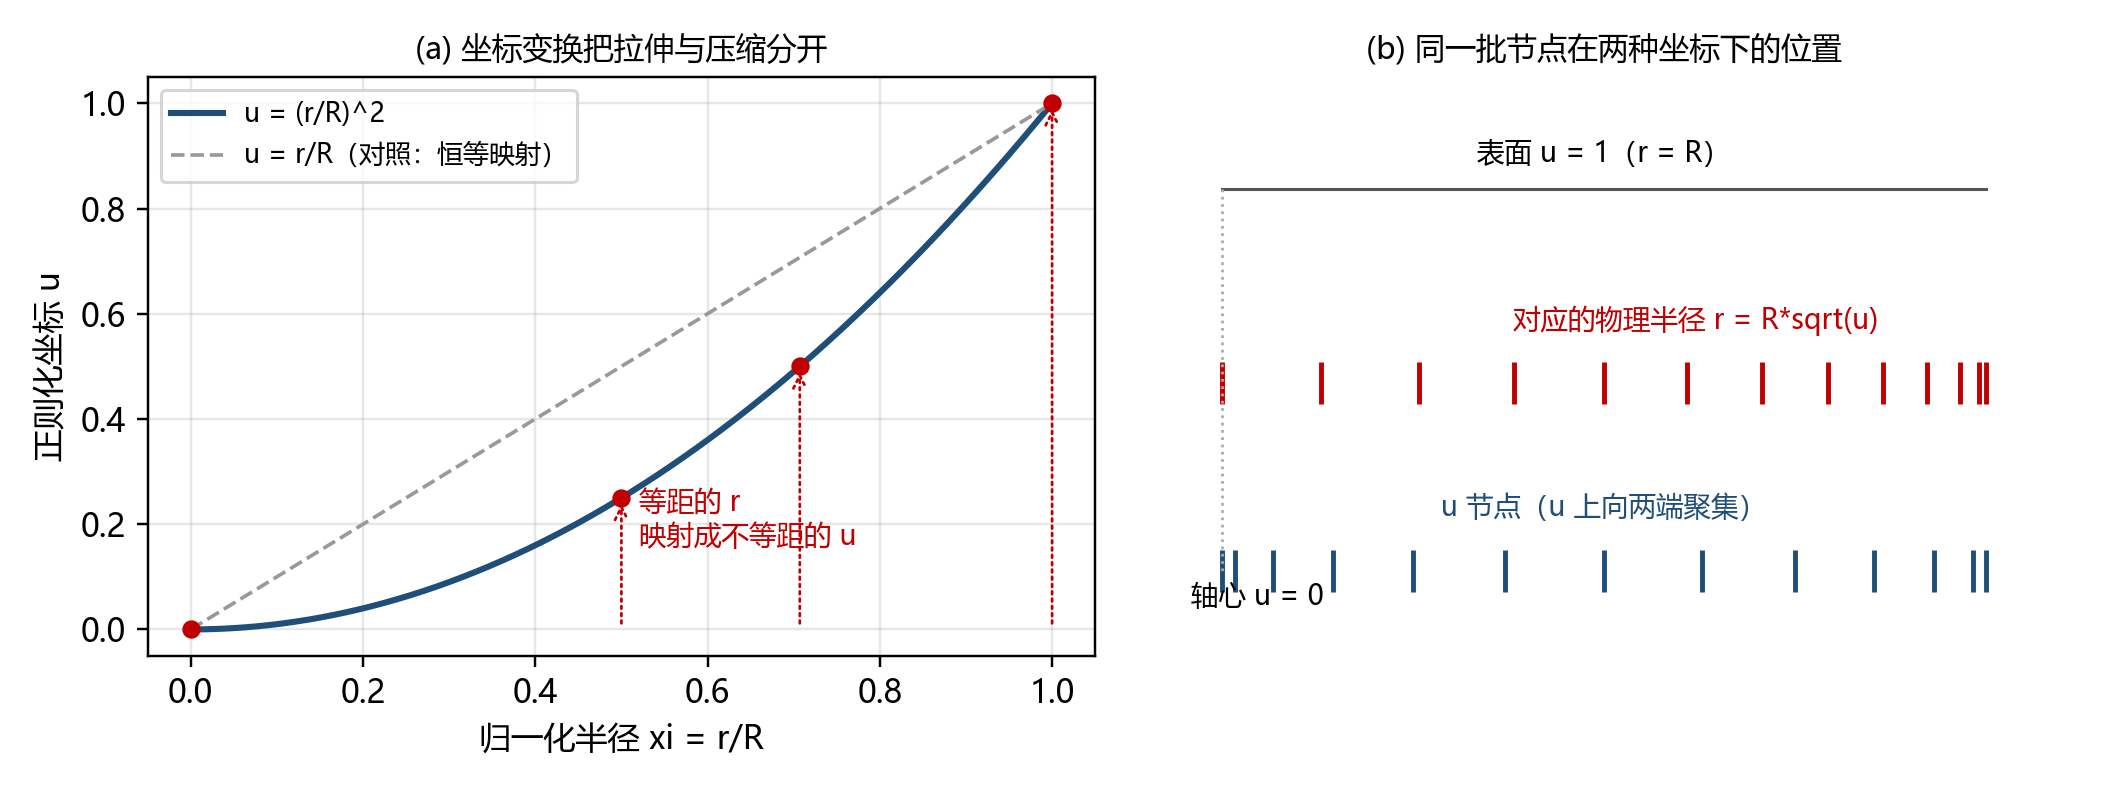
\includegraphics[width=\textwidth]{fig_map.png}
\caption{坐标变换 $u=(r/R)^2$ 的几何意义。
左图是变换曲线，右图是同一批节点在两种坐标下的位置。}
\end{figure}

\subsection{这张图回答什么疑问}

为什么要把半径换成半径的平方。这张图回答两件事：
变换对距离做了什么，以及同一批节点在新坐标下落在哪里。

\subsection{画的是什么}

左图画两条曲线。一条是 $u=\xi^2$，另一条是恒等映射 $u=\xi$ 作对照。
横轴是归一化半径，纵轴是坐标 $u$。
图上标了四个点并画了虚线，把横轴上的等距位置对应到纵轴上的值。

右图画两行刻度。上一行是把切比雪夫节点换算到 $u$ 坐标后的位置，
下一行是把同一批节点开平方换算回物理半径后的位置。

\subsection{数据从哪来}

这是示意图，数据由公式直接算出。
左图取四组对应关系：半径比零对应 $u$ 等于零，
半径比零点五对应 $u$ 等于零点二五，
半径比零点七零七对应 $u$ 等于零点五，
半径比一对应 $u$ 等于一。

右图取节点数十二，用切比雪夫高斯洛巴托节点公式 $x_j=\cos(j\pi/N)$
算出十三个 $x$，再换算成 $u=(1-x)/2$，最后开平方得到半径比。

\subsection{逐要素读图}

\begin{itemize}[leftmargin=1.6em]
\item 左图的两条曲线在原点与右上角相交，其余位置不重合。
\item 左图曲线上方的区域对应半径比小于一，$u$ 始终不超过半径比，
      说明变换把区间前半段压缩、后半段拉伸。
\item 右图上一行的刻度在两端明显变密，这是切比雪夫节点的固有分布。
\item 右图下一行的刻度整体右移，因为开平方把靠近零的区间拉开了。
\end{itemize}

\subsection{能读出什么}

左图给的是一张对应表，可以这样理解：
物理上等距的四个位置，
在 $u$ 坐标里分别落在零、零点二五、零点五、一，
也就是被重新分配成了后半段更疏、前半段更挤的分布。

这个重新分配有一个直接好处。
从轴心到半径百分之七十的位置，占了一半的 $u$ 区间，
而这段区域恰好是解变化平缓的区域；
从半径百分之七十到表面，占了另一半 $u$ 区间，
而这正是解变化最剧烈的表层。
变换把一半的离散点自动分给了最需要分辨的表层。

\subsection{能证明什么，不能证明什么}

这张图能说明变换对区间的重新分配，以及为什么这种分配对本题有利。

它不能说明变换消除了轴心的奇异。
那件事靠的是代数恒等式，与图无关：
在 $u$ 坐标下算子写成 $(4/R^2)\,\partial_u(u\,D\,\partial_u C)$，
$u$ 等于零时方括号里的量有限，奇异消失。
这一步要在讲解稿第二部分第五章看推导，不是看图。

\subsection{生成代码}

\begin{lstlisting}
N = 12
j = np.arange(N + 1)
x = np.cos(np.pi * j / N)
u = (1 - x) / 2
rnodes = np.sqrt(u)
b.plot(u, np.zeros_like(u), "|", color="#1f4e79", ms=14, mew=1.6)
b.plot(rnodes, np.ones_like(u) * 0.55, "|", color="#c00000", ms=14, mew=1.6)
\end{lstlisting}

第 1 行到第 3 行按公式算出十三个切比雪夫节点。
第 4 行把节点从 $[-1,1]$ 映射到 $[0,1]$，这就是坐标 $u$。
第 5 行开平方得到对应的物理半径比。
第 6 行与第 7 行把两批位置画成上下两行刻度，
用竖线符号加粗，便于比较疏密。

\subsection{容易读错的地方}

容易误以为 $u$ 就是半径。它不是，
$u$ 是半径比值的平方，取值从零到一，没有长度量纲。
换算回物理位置要用 $r=R\sqrt{u}$。

也容易误以为图上的节点就是计算节点。
这张图用了十二个节点是为了画得清楚，
实际生产计算用的是六十四个节点。

% =====================================================================
\section{图 4：切比雪夫节点的来源}

\begin{figure}[H]
\centering
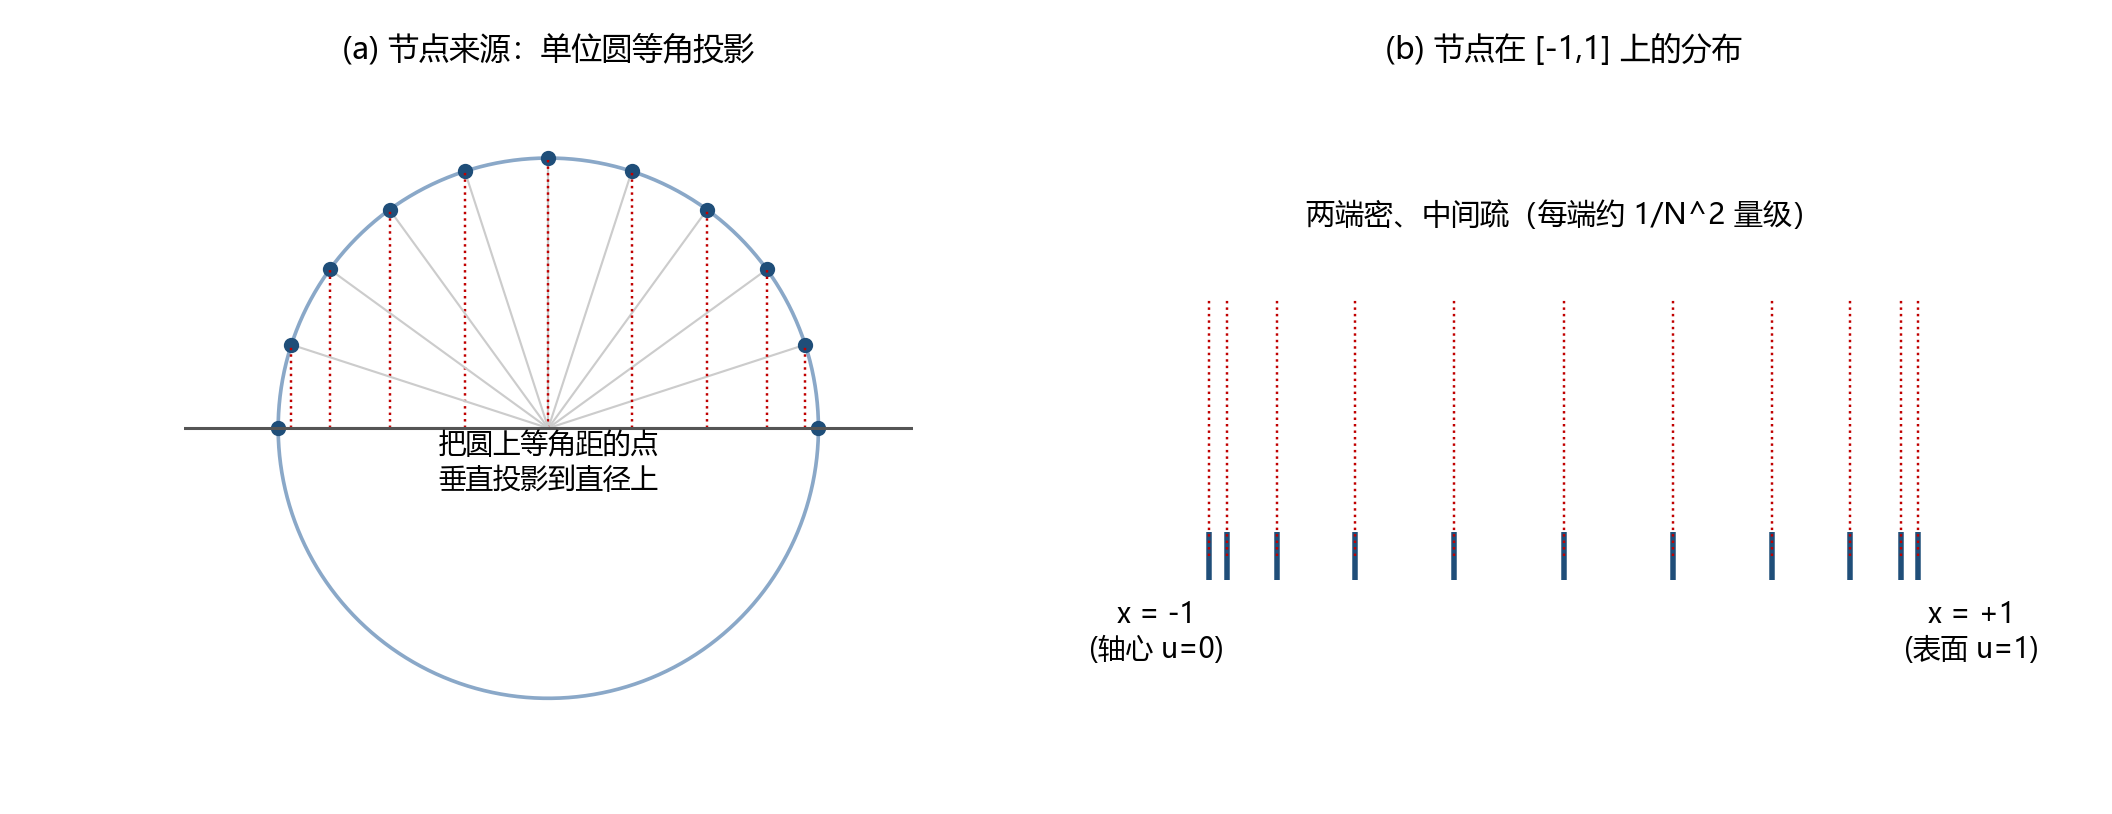
\includegraphics[width=\textwidth]{fig_cheb.png}
\caption{切比雪夫高斯洛巴托节点的来源。
左图在单位圆上按等角距取点，再垂直投影到直径上；
右图是投影结果在区间上的分布。}
\end{figure}

\subsection{这张图回答什么疑问}

节点为什么不用等距的，而要用余弦分布。
这张图给出一个可以自己动手验证的构造方法。

\subsection{画的是什么}

左图画一个单位圆，从圆心引出十一条半径，
每条半径与圆的交点画一个实心点，再从该点向水平直径作垂线。
垂足就是节点位置。
右图把这些垂足单独画成一行刻度，并用虚线标出它们的不均匀程度。

\subsection{数据从哪来}

这是示意图，纯几何构造。
取节点数十，角度按 $\pi/N$ 等分，共十一个角度。
交点的水平坐标就是 $\cos(j\pi/N)$，这正是节点公式本身。

\subsection{逐要素读图}

\begin{itemize}[leftmargin=1.6em]
\item 左图上圆上的点沿圆周均匀分布，相邻点之间的弧长相等。
\item 左图上的垂线在靠近两端处更密。
\item 右图显示投影结果是两端密、中间疏的分布。
\item 右图两端最外两个节点到端点的距离，与中间相邻节点的间距相比，
      差了大约一个数量级。
\end{itemize}

\subsection{能读出什么}

可以用一个简单公式估计这个差别。
中间相邻节点的间距约为 $\pi/N$，
而最靠端点的那个节点到端点的距离约为 $\pi^2/(2N^2)$。
两者之比是 $2N/\pi$，约等于 $0.64N$。
节点数取六十四时，两端比中间密约四十一倍。

这个公式也解释了另一个常被忽略的事实：
在 $u$ 坐标下，节点间距要再减半，
因为 $u=(1-x)/2$，最小间距变成 $\pi^2/(4N^2)$。
节点数六十四时它是 $6.02\times10^{-4}$，实测值是 $6.023\times10^{-4}$，
两者对得上。

\subsection{能证明什么，不能证明什么}

这张图能说明节点的来源与疏密规律，
以及为什么这种分布在插值里不会产生剧烈摆动。

它不能说明用这些节点就能得到谱精度。
精度还取决于被逼近的函数是否光滑。
本题的解在 $u$ 上是解析函数，这一点在讲解稿第二部分第五章证明，
与节点分布是两件事。

\subsection{生成代码}

\begin{lstlisting}
N = 10
j = np.arange(N + 1)
th = j * np.pi / N
x = np.cos(th)
for jj in range(N + 1):
    a.plot([0, np.cos(th[jj])], [0, np.sin(th[jj])], color="#cccccc", lw=0.7)
    a.plot(np.cos(th[jj]), np.sin(th[jj]), "o", color="#1f4e79", ms=4)
    a.plot([np.cos(th[jj]), np.cos(th[jj])], [0, np.sin(th[jj])],
           ls=":", color="#c00000", lw=0.8)
\end{lstlisting}

第 1 行到第 4 行算出十一个角度以及圆上各点的水平坐标。
第 5 行到第 9 行逐个点画三样东西：
从圆心到圆上的细线、圆上的实心点、以及从圆上垂直落到直径的虚线。
垂足位置就是横坐标，也就是节点。

\subsection{容易读错的地方}

容易把左图的圆当成求解区域。它不是。
本题的求解区域是一维的区间，圆只是构造节点的辅助图形。
真正的一维区间是右图那一条刻度线。

% =====================================================================
\section{图 5：问题三干燥曲线与终点放大}

\begin{figure}[H]
\centering
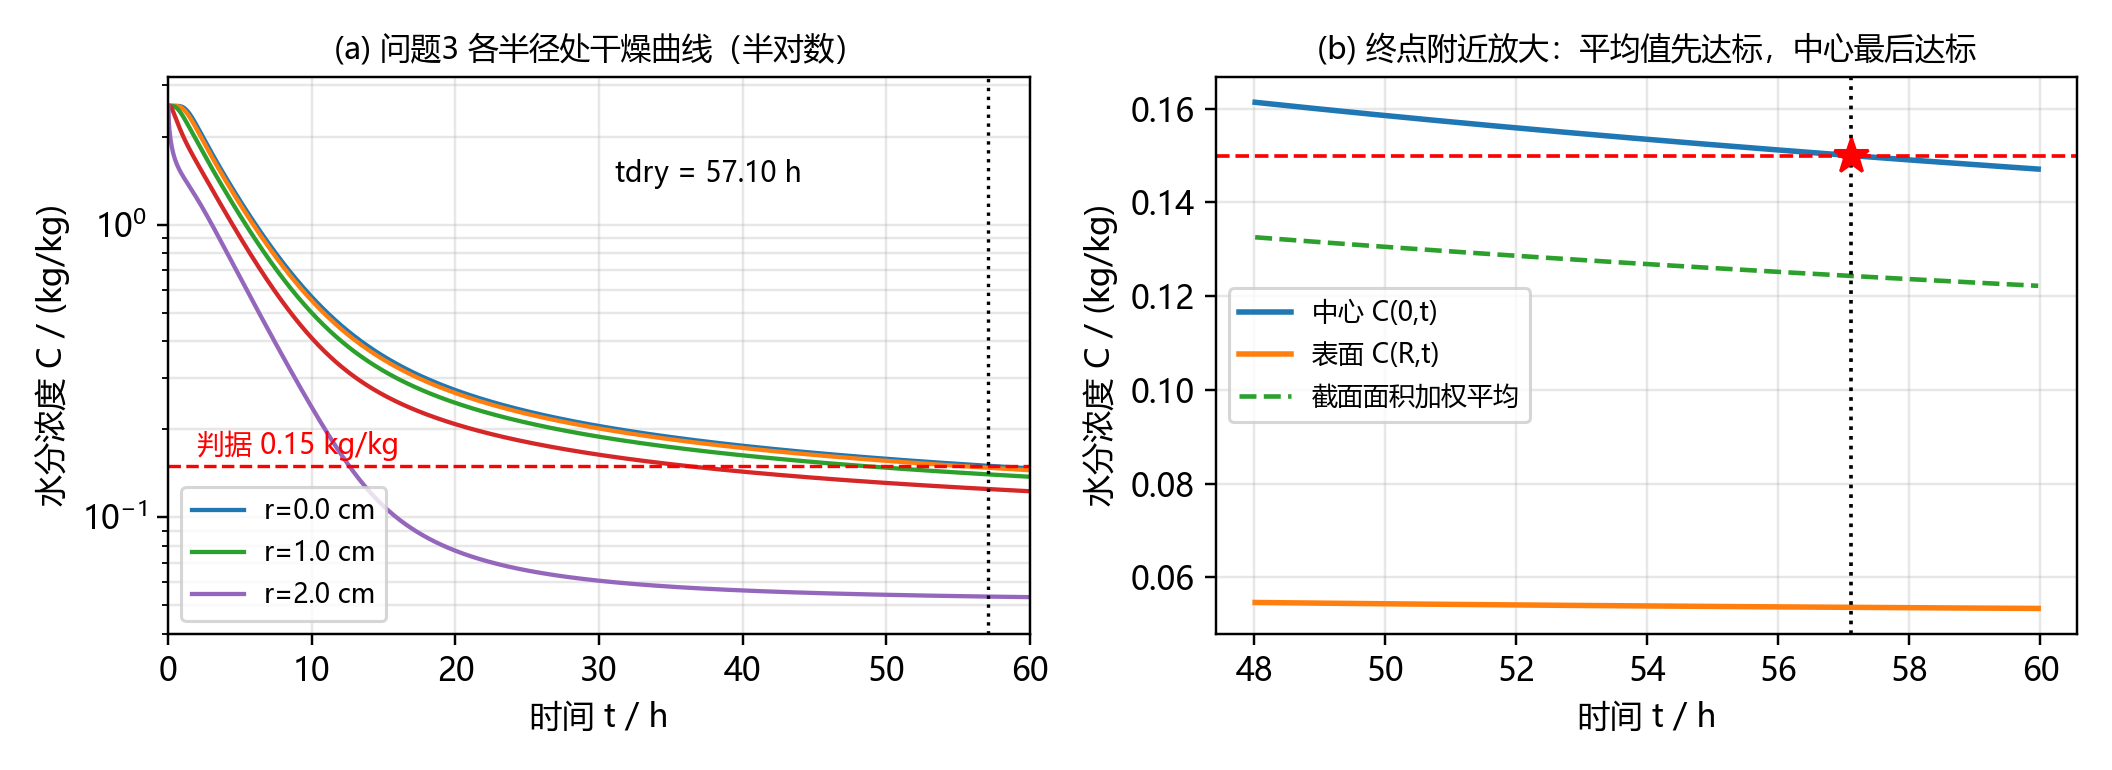
\includegraphics[width=\textwidth]{fig_p3.png}
\caption{问题三的干燥曲线。
左图是五个半径处的水分浓度随时间变化，纵轴取对数；
右图把终点附近放大，并画出截面面积加权平均。}
\end{figure}

\subsection{这张图回答什么疑问}

烘干到底要多久，以及为什么不能用平均值判断。
左图给出全过程，右图给出终点附近的细节。

\subsection{画的是什么}

左图横轴是时间，从零到六十小时，纵轴是水分浓度，取对数刻度。
五条曲线对应五个固定半径。图上有一条红色水平虚线表示判据 $0.15$，
一条黑色竖直点线表示烘干终点。

右图把四十八到六十小时这一段放大，纵轴改回线性刻度。
图上三条曲线分别是中心值、表面值与截面面积加权平均值，
另外用红色星号标出判据与终点的交点。

\subsection{数据从哪来}

数据由主求解器实算，参数是节点数六十四、问题三物性、
相对容差 $10^{-10}$。
先用终端事件求出烘干时刻，得到 $205574.519$ 秒，即 $57.1040$ 小时；
再重新积分到终点的百分之一点零六，输出一千五百个时刻。

右图的截面平均值不是简单地把几条曲线平均。
它的定义是

\begin{equation}
\bar C(t)=\frac{2}{R^2}\int_0^{R}C(r,t)\,r\,\mathrm{d}r ,
\end{equation}

其中权重 $r$ 来自环面积与半径成正比。
脚本先把解插值到四百零一个均匀半径点，再按这个式子做梯形积分。
这一步的做法在第十节展开说明，那里也是本次画图时真正踩到的坑。

\subsection{逐要素读图}

\begin{itemize}[leftmargin=1.6em]
\item 左图五条曲线从下到上依次是表面、一点五、一、零点五厘米与中心。
      表面最低，因为那里最先失水。
\item 左图在十到二十小时之间曲线出现明显转折，
      这是扩散系数随含水率下降而急剧变小的结果。
\item 左图中心那条曲线直到五十小时以后才靠近判据线。
\item 右图三条曲线里，平均值最先穿过判据线，中心最后穿过。
\item 右图红色星号落在中心曲线与判据线的交点上，
      这个交点对应的时间就是烘干时长。
\item 右图横轴的终点处，表面值已经降到零点零五左右，
      远低于判据，说明烘干的瓶颈在中心。
\end{itemize}

\subsection{能读出什么}

几个时刻的读数如下，单位是千克每千克。

\begin{center}
\begin{tabular}{@{}lrrrrr@{}}
\toprule
时刻 / 小时 & 中心 & 0.5 厘米 & 1.0 厘米 & 1.5 厘米 & 表面 \\
\midrule
6 & 1.01210 & 0.98354 & 0.89772 & 0.75254 & 0.53237 \\
12 & 0.45499 & 0.44209 & 0.40223 & 0.32932 & 0.16531 \\
24 & 0.23711 & 0.23207 & 0.21614 & 0.18511 & 0.06735 \\
36 & 0.18527 & 0.18194 & 0.17128 & 0.14996 & 0.05752 \\
48 & 0.16137 & 0.15874 & 0.15028 & 0.13310 & 0.05463 \\
终点 & 0.15001 & 0.14769 & 0.14022 & 0.12492 & 0.05359 \\
\bottomrule
\end{tabular}
\end{center}

从这张表可以读出三件事。

第一，表面早已干透。十二小时时表面已经降到零点一六五，
之后一直在下降，但下降越来越慢，因为扩散系数随含水率下降而变小。

第二，中心最后达标。终点时刻全场最大值出现在中心，恰好等于判据。

第三，截面面积加权平均值在 $35.9$ 小时就低于判据，
比中心达标早了二十一点二小时。
如果用平均值当判据，会把烘干时间低估约百分之三十七。

\begin{keypoint}
判据必须取全场的最大值，不能取平均值，也不能取表面值。
表面最先干，平均值受表层拖累而偏小，两者都会低估烘干时间。
\end{keypoint}

\subsection{能证明什么，不能证明什么}

这张图能说明干燥的推进方式：表面先干，干燥前沿向内移动，
中心最后达标。它也能说明为什么判据要写成全场最大值小于阈值。

它不能回答数值精度问题。
图上没有任何误差信息，终点时刻的可靠性要用收敛性和多方法互证回答，
那是图 7 与讲解稿第四部分的内容。

\subsection{容易读错的地方}

左图纵轴是对数刻度，所以曲线看起来比较平缓，
容易误以为后期含水率下降得很慢。
实际上从十二小时的零点四六降到终点的零点一五，
绝对降幅并不小，只是在对数轴上被压缩了。

右图的三条曲线在不同的横轴范围内都接近直线，
容易误以为变化速率是常数。
线性刻度下看斜率才是真实的速率，
因此在终点附近做线性放大是有必要的。

还有一点是关于平均值曲线。
这条曲线是本次重新计算过的：
最初画图时用的是几个采样点的算术平均，
那会把平均值压到零点二以下，达标时刻提前到二十六个小时。
按面积加权重新算以后，达标时刻是 $35.9$ 小时。
两种画法在同一张图上差了一个多小时，读者无法从图上分辨，
所以必须交代清楚用的是哪一种。第十节给出对比数据。

\subsection{生成代码}

\begin{lstlisting}
def ev3(t, y):
    return np.max(y[:s3.Np]) - CRIT
ev3.terminal = True
ev3.direction = -1
solE = s3.solve(300000.0, rtol=1e-10, atol=at3, events=ev3)
tdry3 = float(solE.t_events[0][0])
\end{lstlisting}

第 1 行到第 2 行定义监视函数，
它返回全场含水率最大值与判据之差。
第 3 行告诉积分器找到零点就停止。
第 4 行给出穿过方向为负，也就是只在数值下降穿过零时才触发。
第 5 行求解，视界给到三十万秒。
第 6 行从结果里取出事件时刻。

\begin{lstlisting}
rr = np.linspace(0.0, cm.R0, 401)
wb = (-1.0) ** np.arange(s3.Np)
wb[0] *= 0.5
wb[-1] *= 0.5
dif = (rr / cm.R0)[:, None] ** 2 - s3.u[None, :]
den = (wb[None, :] / np.where(np.abs(dif) < 1e-14, 1.0, dif)).sum(axis=1, keepdims=True)
Bm = (wb[None, :] / np.where(np.abs(dif) < 1e-14, 1.0, dif)) / den
Cf = Bm @ sol3.y[:s3.Np, :]
meanC = np.trapezoid(Cf * rr[:, None], rr, axis=0) * 2.0 / cm.R0 ** 2
\end{lstlisting}

第 1 行在物理半径上取四百零一个均匀点。
第 2 行到第 4 行构造重心插值的权重：
切比雪夫高斯洛巴托节点的权重是正负一交替，两个端点各取一半。
第 5 行算出插值点与节点在 $u$ 坐标下的距离矩阵。
第 6 行到第 7 行按重心插值公式组装插值矩阵，
分母加一个判断是为了避免正好落在节点上时除零。
第 8 行把全部时刻的解一次性插值到均匀半径网格。
第 9 行按面积加权做梯形积分，乘以前面的系数完成截面平均。

\subsection{容易读错的地方}

右图那条虚线容易被当成简单算术平均。
它不是，它是按面积加权的积分平均，权重是半径。
两者在本图上差很多，第十节给出具体数字。

% =====================================================================
\section{图 6：通量形式的谱配置}

\begin{figure}[H]
\centering
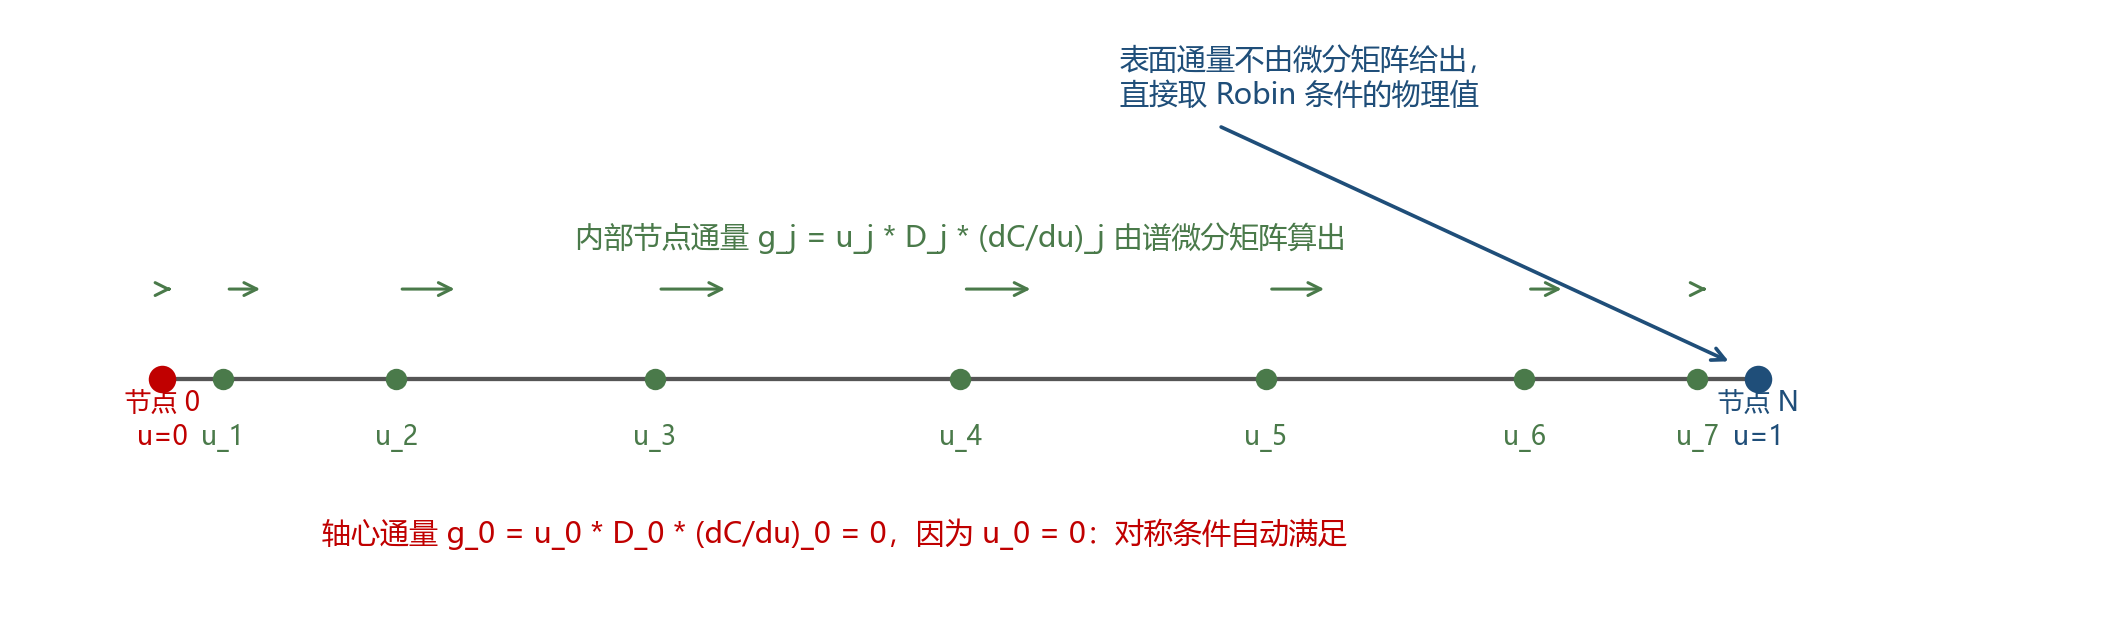
\includegraphics[width=\textwidth]{fig_flux.png}
\caption{通量形式的谱配置。
内部节点的通量由谱微分矩阵算出，表面节点的通量直接取物理边界条件，
轴心节点的通量因为权重为零而自动为零。}
\end{figure}

\subsection{这张图回答什么疑问}

离散方程写成通量形式是什么意思，边界条件是怎么进到方程里的。

\subsection{画的是什么}

图中间是一条横轴，代表坐标 $u$ 从零到一。
轴上画了九个节点，其中最左一个是轴心，最右一个是表面，
中间七个是内部节点。
内部节点之间画了箭头表示通量，上方文字说明内部通量由谱微分矩阵算出。
右上角文字与箭头指向表面节点，
说明表面通量不由微分矩阵给出，而直接取边界条件的物理值。
下方文字说明轴心通量恒等于零及其原因。

\subsection{数据从哪来}

这是概念示意图，不含求解器输出。
节点位置按切比雪夫节点公式取节点数八算出，
用它只是为了画得稀疏一些。

\subsection{逐要素读图}

\begin{itemize}[leftmargin=1.6em]
\item 轴心节点画成红色，标注 $u$ 等于零。
\item 表面节点画成深蓝色，标注 $u$ 等于一。
\item 中间节点画成绿色，标注为第一到第七个内部节点。
\item 每个内部节点上方有一个向右的箭头，代表该处的通量。
\item 上方文字写出通量的定义：节点值乘以扩散系数再乘以导数的谱近似。
\item 右上文字指出表面通量另行取值。
\item 下方文字给出轴心通量为零的等式与原因。
\end{itemize}

\subsection{能读出什么}

这张图对应离散方程里的三件事，可以逐条对照代码。

第一，内部节点的通量由谱微分矩阵与节点值的乘积算出，
写成 $g_j=u_jD_j(\mathrm{D}_uC)_j$，
其中 $\mathrm{D}_u$ 是微分矩阵，$u_j$ 是节点坐标，$D_j$ 是该节点的扩散系数。

第二，表面节点的通量不这样算，
而是由边界条件直接给出：$g_N=\frac12 h_m R\,(C_{\mathrm{air}}-C_N)$。
这个式子里的二分之一来自坐标变换时链式法则产生的因子，在讲解稿里有推导。

第三，轴心节点的通量是 $g_0=u_0D_0(\mathrm{D}_uC)_0$，
而 $u_0$ 等于零，所以整个乘积等于零。
这不是近似，是恒等式，对称条件因此自动满足，不需要额外处理。

\subsection{能证明什么，不能证明什么}

这张图能说明通量形式的三段结构，
以及为什么轴心不需要特殊边界条件、表面条件又必须单独处理。

它不能证明这样处理以后精度仍然很高。
那一点要用数值实验回答：谱解与闭式解在全场比较，
误差随节点数的变化见图 7 左图。

\subsection{容易读错的地方}

容易以为箭头表示水流方向。
它表示的是离散方程里相邻节点之间传递的量，
在数学上是通量，在物理上确实对应水分与热量的流动方向，
但图上箭头的疏密与长短没有定量含义。

也容易以为轴心通量为零是因为对称性被当作条件加了进去。
实际原因是权重 $u$ 在那里等于零，
对称性是被方程本身包含的，不需要额外声明。

% =====================================================================
\section{图 7：两种离散方式的收敛对比}

\begin{figure}[H]
\centering
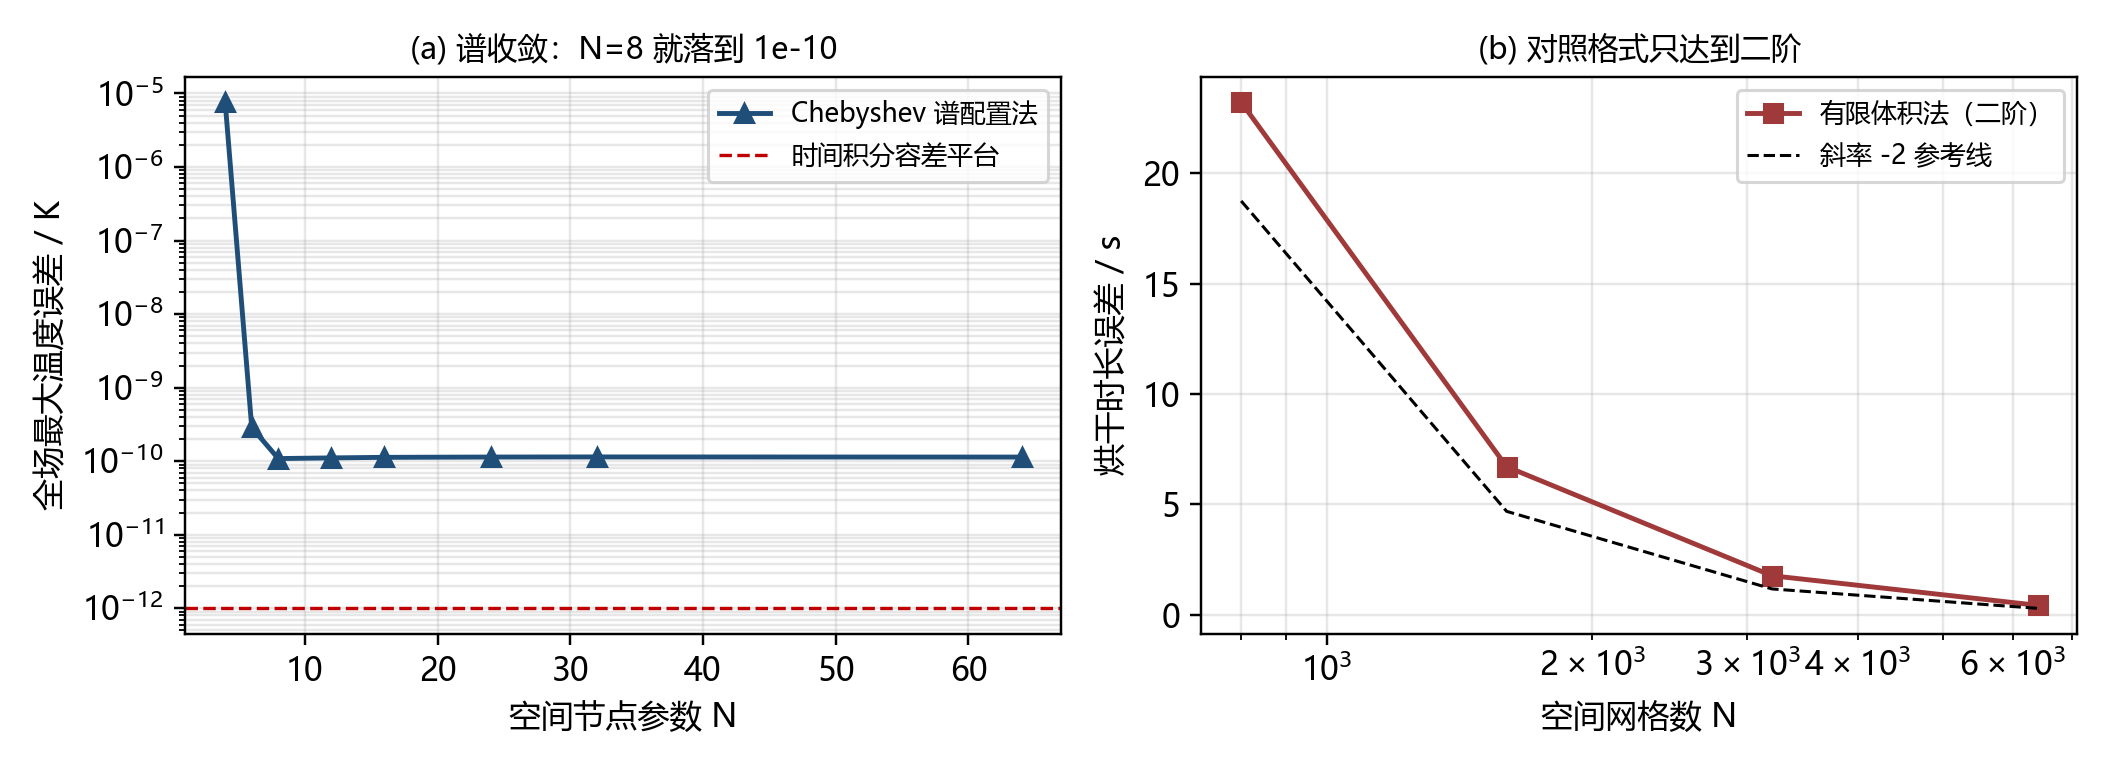
\includegraphics[width=\textwidth]{fig_conv.png}
\caption{两种离散方式的空间收敛。
左图是谱配置法误差随节点数的变化，右图是对照格式的烘干时长误差随网格数的变化。}
\end{figure}

\subsection{这张图回答什么疑问}

谱方法说的精度高到底高在哪里，与常规方法差多少。

\subsection{画的是什么}

左图的横轴是节点参数，纵轴是全场最大温度误差，取对数刻度。
曲线上的方块是八个节点参数下的实测误差，
水平虚线标出时间积分容差造成的平台。

右图的横轴是空间网格数，纵轴是烘干时长误差，都取对数刻度。
曲线上的方块是四组数据，黑色虚线是斜率负二的参考线。

\subsection{数据从哪来}

左图的数据是本次实算。
对八个节点参数分别求解问题一，时间容差固定为 $10^{-12}$，
再把解与闭式解在两百零一个半径点上逐点比较，取最大偏差。

右图的数据不是本次实算，而是取自既有的专家报告第九章第三节。
原因是对照格式要跑到网格数六千四百、时间步一秒、
总时长二十万秒，计算量很大，
不适合在画图脚本里现算。
图上那条斜率负二的参考线是为了显示该格式的收敛阶。
这一点必须交代清楚，否则读者会以为四条数据也是本次跑出来的。

\subsection{逐要素读图}

\begin{itemize}[leftmargin=1.6em]
\item 左图最左边两个点之间落差了四个数量级，
      节点数从四加到六，误差从 $7.59\times10^{-6}$ 掉到 $2.88\times10^{-10}$。
\item 左图从第三个点起变成一条水平线，稳定在 $1.1\times10^{-10}$ 附近。
\item 左图的水平虚线与这条水平线重合，说明平台由时间容差决定。
\item 右图四个点随网格数增加单调下降，且下降速度与参考线大致平行。
\item 右图最右边那个点的误差已经降到一秒以下。
\end{itemize}

\subsection{能读出什么}

左图的读数如下。

\begin{center}
\begin{tabular}{@{}lcccccccc@{}}
\toprule
节点数 & 4 & 6 & 8 & 12 & 16 & 24 & 32 & 64 \\
\midrule
最大误差 / 开尔文 & $7.59\times10^{-6}$ & $2.88\times10^{-10}$ & $1.09\times10^{-10}$
& $1.11\times10^{-10}$ & $1.13\times10^{-10}$ & $1.14\times10^{-10}$
& $1.14\times10^{-10}$ & $1.14\times10^{-10}$ \\
\bottomrule
\end{tabular}
\end{center}

这张表要分两段读。

第一段是前两列。只多两个节点，误差掉了四个多数量级。
这就是谱收敛的样子：不是按固定阶数慢慢降，
而是每增加一点节点数就跳一个台阶。
原因是插值多项式用了所有节点的信息，
而被逼近的函数在 $u$ 坐标下是解析函数。

第二段是后六列。误差不再下降，稳定在 $1.1\times10^{-10}$。
这一段不能再当作方法精度的证据，
因为此时限制精度的是时间积分，不是空间离散。
把时间相对容差从 $10^{-8}$ 收到 $10^{-12}$，
误差依次是 $1.03\times10^{-7}$、$2.34\times10^{-9}$、$1.14\times10^{-10}$，
与容差同步变化，这就证明了平台的来源。
顺带说，双精度浮点数在温度三十四附近的表示间隔约为 $10^{-14}$ 开尔文，
比这个平台还小四个数量级，所以平台不是计算机的表示极限。

右图的读数如下，单位是秒。

\begin{center}
\begin{tabular}{@{}lcccc@{}}
\toprule
空间网格数 & 800 & 1600 & 3200 & 6400 \\
\midrule
烘干时长 & 205550.98 & 205567.49 & 205572.43 & 205573.77 \\
与 205574.2 之差 & 23.22 & 6.71 & 1.77 & 0.43 \\
相邻差之比 & --- & 3.46 & 3.79 & 4.12 \\
\bottomrule
\end{tabular}
\end{center}

网格数每翻一倍，误差降到约四分之一，也就是四倍左右，
这正是二阶收敛的特征。斜率负二的参考线与数据点大致平行。

两相对照可以看出差别：对照格式要把网格从八百加密到六千四百，
相差八倍，才把误差从二十三秒压到零点四秒；
而谱方法只用七个节点就把空间误差压到了时间误差之下。

\subsection{能证明什么，不能证明什么}

这张图能说明两件事：
谱方法在很少的节点下就能达到很高精度；
对照格式只达二阶，需要密集网格。

它不能说明烘干时长本身已经完全可靠。
烘干时长是对时间极度敏感的量，还要做时间方向的收敛检验，
那是讲解稿第四部分与第九节的内容。

\subsection{容易读错的地方}

最容易读错的是左图后半段那条水平线。
它看起来像收敛停滞，实际上是误差已经被时间误差盖住。
如果不看容差检验的那三个数，很容易得出错误结论，
以为谱方法在节点数较多时失效。

另一个容易读错的地方是右图的数据出处。
它不是本次实算，而是引用既有报告。
本文把它放进来是为了显示收敛阶，
引用时必须在图注或正文里写明来源，
否则会误导读者以为这是本次跑出来的结果。

\subsection{生成代码}

左图的数据这样生成：

\begin{lstlisting}
Ns = [4, 6, 8, 12, 16, 24, 32, 64]
err = []
for N in Ns:
    s = HerbSolver(N, prob=1)
    at = np.concatenate([np.full(s.Np, 1e-14), np.full(s.Np, 1e-12)])
    sol = s.solve(1800.0, t_eval=[1800.0], rtol=1e-12, atol=at)
    rc = np.linspace(0, cm.R0, 201)
    Ti = s._bary(sol.y[s.Np:, -1], (rc / cm.R0) ** 2)
    Te = an.T_exact(rc, 1800.0)
    err.append(float(np.max(np.abs(Ti - Te))))
\end{lstlisting}

第 1 行给出八个节点参数。
第 3 行到第 4 行对每个节点参数建立问题一的求解器，
其中温度绝对容差取 $10^{-12}$、含水率取 $10^{-14}$，
把时间误差压到最低，好让空间误差显出来。
第 5 行求解到一千八百秒，只输出终点一个时刻。
第 6 行取两百零一个半径位置作为比较点。
第 7 行把节点解插值到这些位置，注意自变量是 $u$，所以要取半径比的平方。
第 8 行调用闭式解算出同一点的参考值。
第 9 行取差值的最大绝对值作为误差。

\subsection{容易读错的地方}

左图的横轴是线性刻度而纵轴是对数刻度，
所以前两个点之间的落差在视觉上被夸张了。
实际落差是四个数量级，图上看像是六到七个数量级的高度差，
那是因为对数轴每个刻度代表十倍。

% =====================================================================
\section{读图时最容易踩的三个坑}

上面各节提到的读图陷阱可以归成三类。
这三类都在本次画图过程中真实出现过，写出来供参考。

\subsection{第一个坑：平均值不等于截面平均}

图 5 右图那条虚线最初画错了。
当时的写法是把五个采样半径上的值直接求算术平均：

\begin{lstlisting}
meanC = C3.mean(axis=1)          # 错误做法
\end{lstlisting}

这样算出来的曲线明显偏低，达标时刻是 $26.1$ 小时。
原因是五个采样点等距分布，而真正的截面平均要按面积加权，
权重是半径本身，靠外的点权重更大。
表面附近的值最低，等距平均会给表层过高权重。

正确的定义是

\begin{equation}
\bar C(t)=\frac{2}{R^2}\int_0^{R}C(r,t)\,r\,\mathrm{d}r .
\end{equation}

改用正确的积分以后，达标时刻是 $35.9$ 小时。
两种算法的对比数据如下，单位是千克每千克。

\begin{center}
\begin{tabular}{@{}lccc@{}}
\toprule
时刻 / 小时 & 错误做法：节点直接加权 & 正确做法：谱积分 & 正确做法：半径网格积分 \\
\midrule
6 & 0.697556 & 0.780498 & 0.780497 \\
12 & 0.284031 & 0.335711 & 0.335710 \\
24 & 0.157023 & 0.185335 & 0.185333 \\
36 & 0.128728 & 0.149598 & 0.149596 \\
48 & 0.115148 & 0.132531 & 0.132530 \\
达标时刻 / 小时 & 26.121 & 35.845 & 35.845 \\
\bottomrule
\end{tabular}
\end{center}

表中后两列是用两种完全不同的积分方法算的：
一列用切比雪夫节点上的 Clenshaw-Curtis 权重，
另一列先插值到均匀半径网格再做梯形积分。
两者最大相差 $2.4\times10^{-6}$，互为验证。
第一列与它们的差别达到 $0.2$，说明节点直接加权确实错了。

这里还有一个更细的坑，值得单独提醒。
如果读者拿交付文件 result3.xlsx 自己复核这个积分，
会得到 $35.2$ 小时，而不是 $35.8$ 小时。
原因是该文件只给出二十一个半径列，
用二十一个点做梯形积分，在表面附近精度不够。
把积分点数加到四百零一个，结果就收敛到 $35.8$ 小时。
具体数列如下。

\begin{center}
\begin{tabular}{@{}lccc@{}}
\toprule
积分所用半径点数 & 21 & 401 & 2001 \\
\midrule
达标时刻 / 小时 & 35.18 & 35.83 & 35.83 \\
\bottomrule
\end{tabular}
\end{center}

所以在讲解稿里，正文取的是收敛值 $35.9$ 小时，
并把二十一点给出 $35.2$ 小时这件事一并写明，
免得读者自己一算对不上，反而以为正文写错了。

\subsection{第二个坑：平台不等于精度极限}

图 7 左图后半段那条水平线，最初被解释成计算机能表示的极限。
这个解释是错的，而且与同一段的另一句话自相矛盾，
因为那段文字紧接着说误差是时间积分造成的。
正确做法是把三档容差的数据列出来对照，
用数据说明平台的来源，
再补一句双精度在温度三十四附近的表示间隔约为 $10^{-14}$ 开尔文，
让读者知道真正的表示极限在哪里。

\subsection{第三个坑：图上没标出处的数据会被当成本次结果}

图 7 右图的四组数据来自既有报告，不是本次实算。
这类数据放进图里有两个风险：
读者以为它是本次跑出来的；以及它与本次数据用了不同协议，
两者混在一张图上比较会产生误导。
处理办法有三条：在画图时于代码里写明来源注释；
在图注或正文里点明出处；在正文里给出该数据的原始协议。

% =====================================================================
\section{怎么重新生成与修改}

\subsection{重新生成}

在讲解稿目录下执行：

\begin{lstlisting}
python figs.py
\end{lstlisting}

脚本会依次生成七张图，打印每张图的名字，
数据图还会打印关键读数，例如烘干时长与截面平均达标时刻。
输出目录是讲解稿目录下的 fig 子目录。
生成完以后重新编译讲解稿两遍，新图就会进入 PDF。

\subsection{修改样式}

全部样式集中在脚本开头，改一处就全局生效。

\begin{center}
\begin{tabular}{@{}lll@{}}
\toprule
想改什么 & 改哪里 & 当前值 \\
\midrule
中文字体 & 脚本开头的字体路径 & 微软雅黑 \\
图像分辨率 & savefig.dpi & 220 \\
基本字号 & font.size & 10.5 \\
负号显示 & \texttt{axes.unicode\_minus} & 关 \\
图幅尺寸 & 各函数里的 figsize & 多为 9.6 乘 3.5 英寸 \\
\bottomrule
\end{tabular}
\end{center}

\subsection{修改数据}

数据图的关键参数也在各函数开头，
例如图 2 的节点数六十四与输出间隔六十秒，
图 5 的节点数六十四与一千五百个输出时刻。
改这些参数会同时改变图与打印出来的读数，
改完记得更新图注里引用的数值。

\subsection{一个建议}

画数据图时，最好让脚本同时打印图上出现的读数。
本次七张图里，凡是数据图都在生成时打印了关键数值，
写文档时可以直接引用，不必再去图上估读。
估读不仅慢，还容易出错，尤其是对数坐标的图。

\end{document}
